\section{АНАЛИЗ РЕЗУЛЬТАТОВ ЭКСПЕРИМЕНТОВ}
В разделе \ref{g1} рассмотрены теоремы, которые давали 
теоретическую оценку
характеристик графов, созданных 
в соответствии с моделью $G(n,p)$. В этом разделе будут 
показаны результаты численного исследования модели  $G(n,p)$.
\subsection{Анализ размеров наибольших компонент связности}
Рассмотрим изменение размеров наибольших компонент связности 
при $n = 10000$, $\epsilon=0.1$, $p \in [\frac{1-\epsilon}{n};\frac{1+\epsilon}{n}]$.
\begin{figure}[H] 
    \centering
    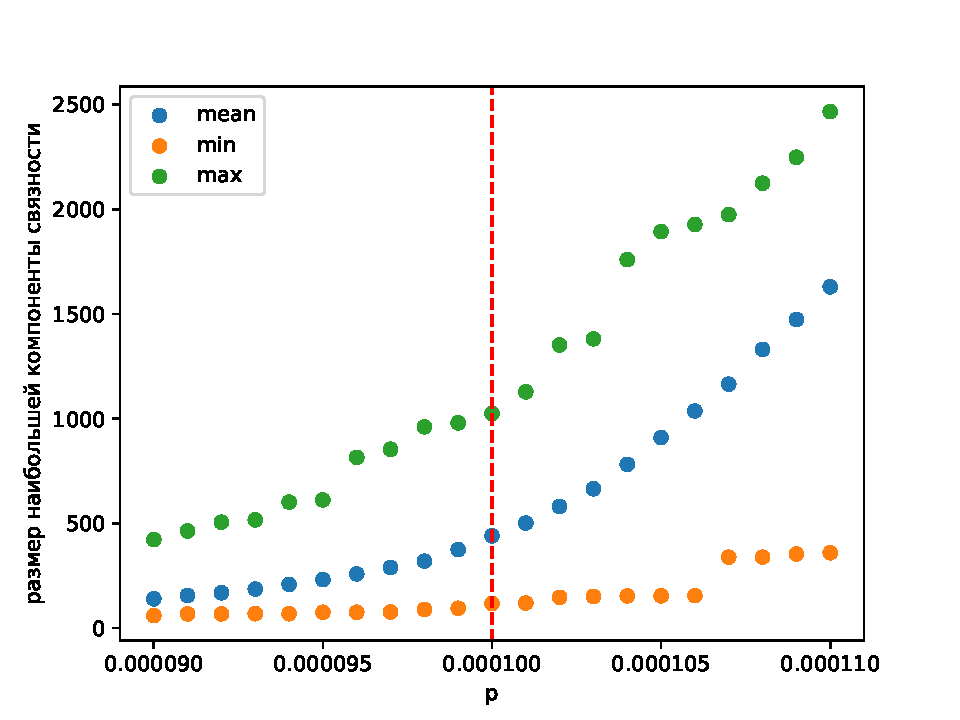
\includegraphics{../../plots/plot.pdf} 
    \caption{Изменение размера наибольшей компоненты связности}
    \label{cmp_1}
\end{figure} 
\begin{figure}[H] 
    \centering
    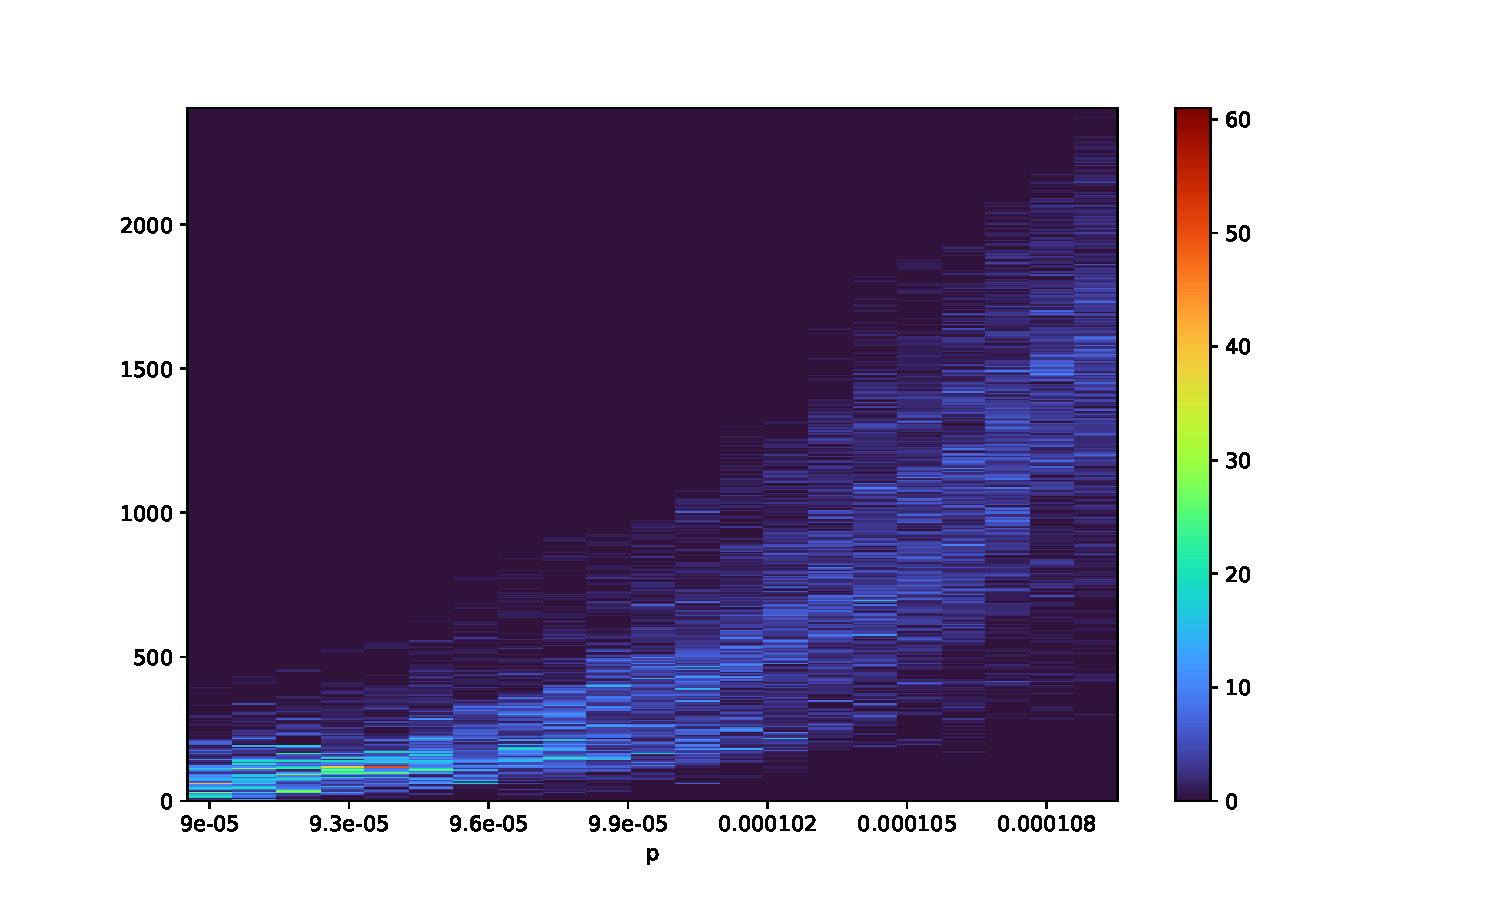
\includegraphics[scale=0.8]{../../plots/hm.pdf} 
    \caption{Тепловая карта изменения размера наибольшей компоненты связности}
    \label{hm_1}
\end{figure} 
% На рисунках \ref{cmp_1},\ref{hm_1} приведена визуализация изменений размера 
% наибольшей компоненты связности.
Из графика, изображенного на рисунке \ref{cmp_1},
можно увидеть фазовый переход в точке $p =\frac{1}{n}$, 
помеченной красной чертой. После его достижения размер наибольших компонент связности начинает расти быстрее. Тепловая 
карта, приведенная на рисунке \ref{hm_1} более подробно описывает
изменения размера наибольшей компоненты связности.

Теперь рассмотрим выполнение теорем о размерах компонент связности при $n=10000$, $\epsilon \in \{0.1,0.5,0.01\}$. Для каждого значения 
$\epsilon$ было проведено 350 экспериментов, вычислены размеры наибольших компонент связности. При $p = \frac{1-\epsilon}{n}$ 
была посчитана доля экспериментов, где размер наибольшей компоненты связности меньше теоретической оценки, при 
$p = \frac{1 + \epsilon}{n}$, доля экспериментов, где размер 
наибольшей компоненты связности больше теоретической оценки.
\begin{table}[H]
    \centering
    \caption{Результаты численного исследования размеров наибольших компонент связности}
    \begin{tabular}{|c|c|c|c|}
        \hline
        $\epsilon$ & $0.1$ & $0.5$ & $0.01$ \\
        \hline
        $p = \frac{1-\epsilon}{n}$ & $1$ &  $1$ &  $1$ \\
        \hline
        $p = \frac{1+\epsilon}{n}$ & $0.94$ & $1$ & $1$ \\
        \hline
    \end{tabular}
    \label{tab_1}
\end{table}
Как можно заметить из таблицы \ref{tab_1}, теоремы о 
размерах компонент связности выполняются почти всегда.
\subsection{Проверка симметричности распределения размера наибольших компонент связности}
\label{test}
Рассмотрим метод проверки гипотезы о симметричности выборки, описанный в статье Мяо, Гель и Гаствирта \cite{sym}.
Построим статистику $T = \frac{\overline{X} - M}{J}$, где:
\begin{enumerate}
    \item $\overline{X}$ -- выборочное среднее;
    \item $M$ -- выборочная медиана;
    \item  $J =  \sqrt{\frac{\pi}{2}} \cdot \frac{1}{n}\sum_{i=1}^{n} |X_{i} - M| $
\end{enumerate}

$H_0$ -- гипотеза о симметричности выборки, отклоняется, если
$|T| \ge \frac{z_{\frac{\alpha}{2}} \sqrt{0.5708} }{\sqrt{n} }$,
где $z_{\alpha}$ -- верхний квантиль уровня $\alpha$ стандартного нормального распределения. Для тестов, приведенных ниже, 
использовался $\alpha = 0.95$
 \begin{figure}[H] 
     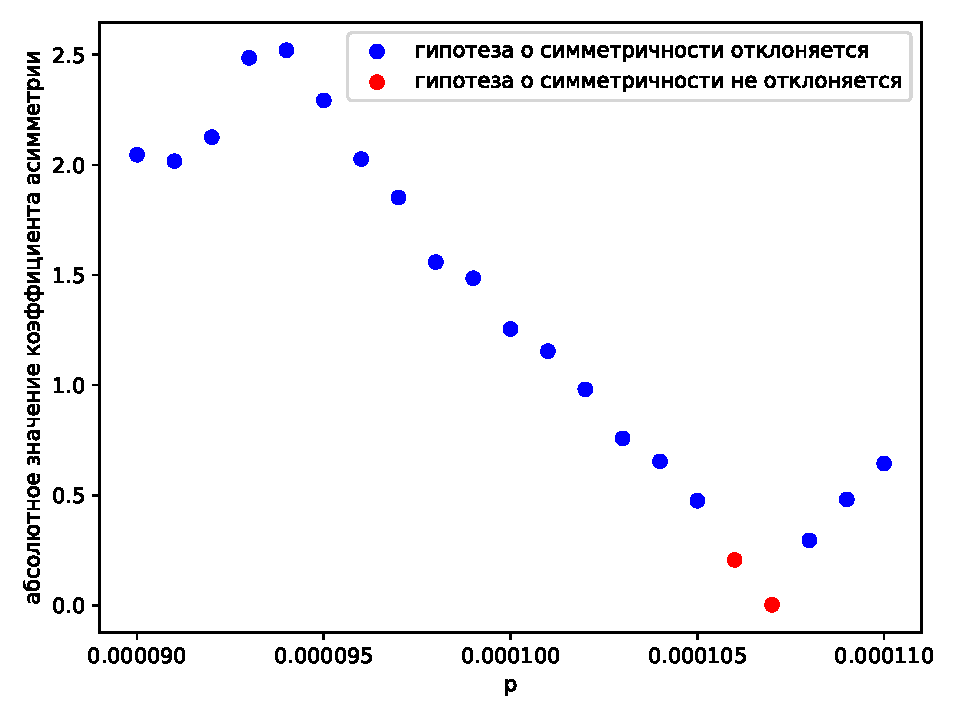
\includegraphics{../../plots/skew_350.pdf} 
     \caption{График изменения абсолютного значения коэффициента асимметрии}
     \label{skew}
\end{figure} 
На рисунке \ref{skew} приведена визуализация вышеописанного 
метода для проверки симметричности распределения размера
наибольшей компоненты связности для модели 
$G(n,p), n =10000, p \in [\frac{1-\epsilon}{n};\frac{1+\epsilon}{n}], \epsilon=0.1$. Как можно заметить 
коэффициент асимметрии значительно отличается от нуля, а 
использование теста только подтверждает отсутствие симметричности.
\subsection{Исследование путей в графах}
Задача поиска самого длинного пути в графе является 
NP-полной, из-за чего оцениваться будет не самый длинный путь, 
а самый длинный найденный путь с помощью поиска в глубину.
Вершины графа, которые находятся в стеке во время 
выполнения поиска в глубину, образуют путь.
\begin{figure}[H] 
    \centering
    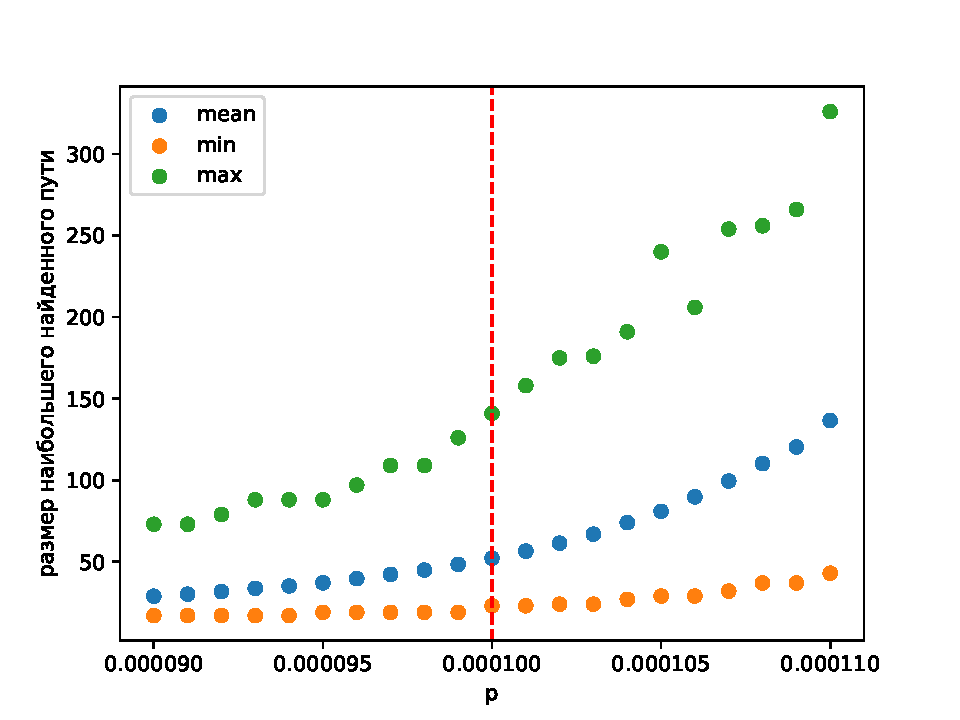
\includegraphics{../../plots/max_path_plot.pdf} 
    \caption{Изменение длины наибольшего найденного пути}
    \label{path_1}
\end{figure} 
\begin{figure}[H] 
\centering
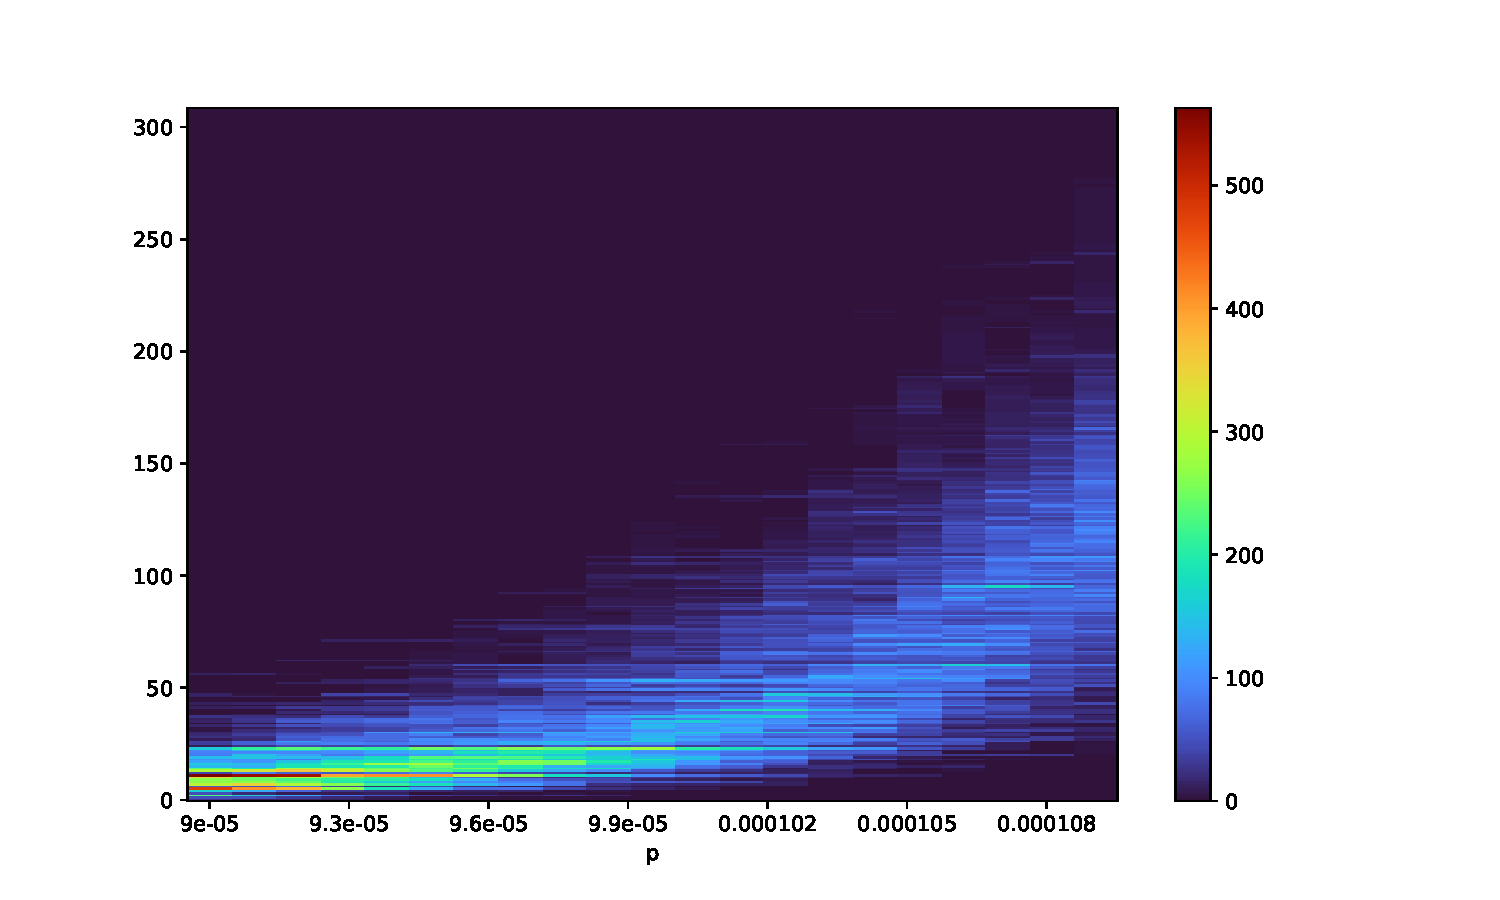
\includegraphics[scale=0.6]{../../plots/hm2.pdf}
\caption{Тепловая карта изменения наибольшего найденного пути}
\label{hm_2}
\end{figure} 
На рисунках \ref{path_1},\ref{hm_2} приведена 
визуализация изменения наибольшего найденного пути 
с помощью поиска в глубину. Графы строились при 
$n = 10000$, $\epsilon =0.1$, $p \in [\frac{1-\epsilon}{n};\frac{1+\epsilon}{n}]$.
На рисунке \ref{path_1} виден характер изменений наибольшего 
найденного пути. Тепловая карта, приведенная на рисунке \ref{hm_2}, описывает более точно характер изменений. Было проведено 350 экспериментов 
при $n = 10000$, $\epsilon \in \{0.1,0.01,0.5\}$. Теорема
об оценке длины найденного пути в графе выполнялась всегда.
\subsection{Проверка длины наибольшего найденного пути на симметричность}
Применим метод проверки выборки на симметричность, описанный в 
разделе \ref{test}. Использовались данные о вычислении 
длины наибольшего найденного пути с помощью поиска в глубину при
$n=10000$,  $\epsilon = 0.1$ , $p \in [\frac{1-\epsilon}{n};\frac{1+\epsilon}{n}]$.
\begin{figure}[H] 
\centering 
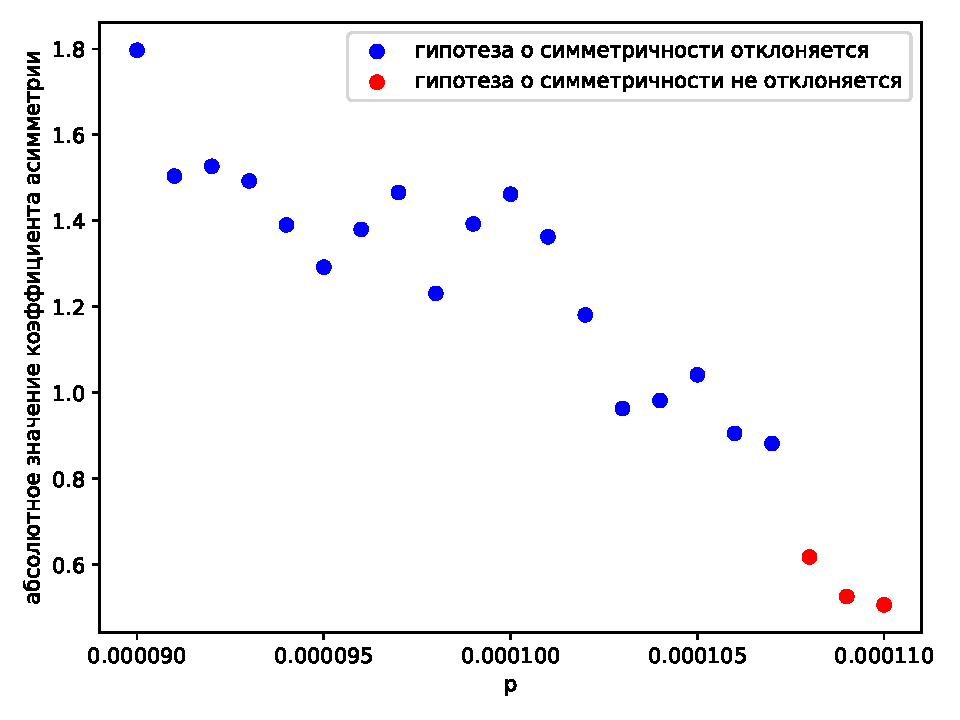
\includegraphics{../../plots/skew_path.pdf}
\caption{Изменение абсолютного значения коэффициента асимметрии}
\label{skew_path}
\end{figure} 
Из графика, представленного на рисунке \ref{skew_path} 
можно заметить, что симметричность в распределении
длин найденных путей не наблюдается.
\subsection{Исследование связности графов}
Были проведены 110 экспериментов, $n=10000$, $p \in [0.1 \frac{\ln{n}}{n} ; 1.2\frac{\ln{n}}{n}]$. Для каждого 
графа вычислялось количество компонент связности. Для 
каждого значения $p$ была вычислена доля связных графов, среди 
всех экспериментов.
\begin{figure}[H] 
    \centering
    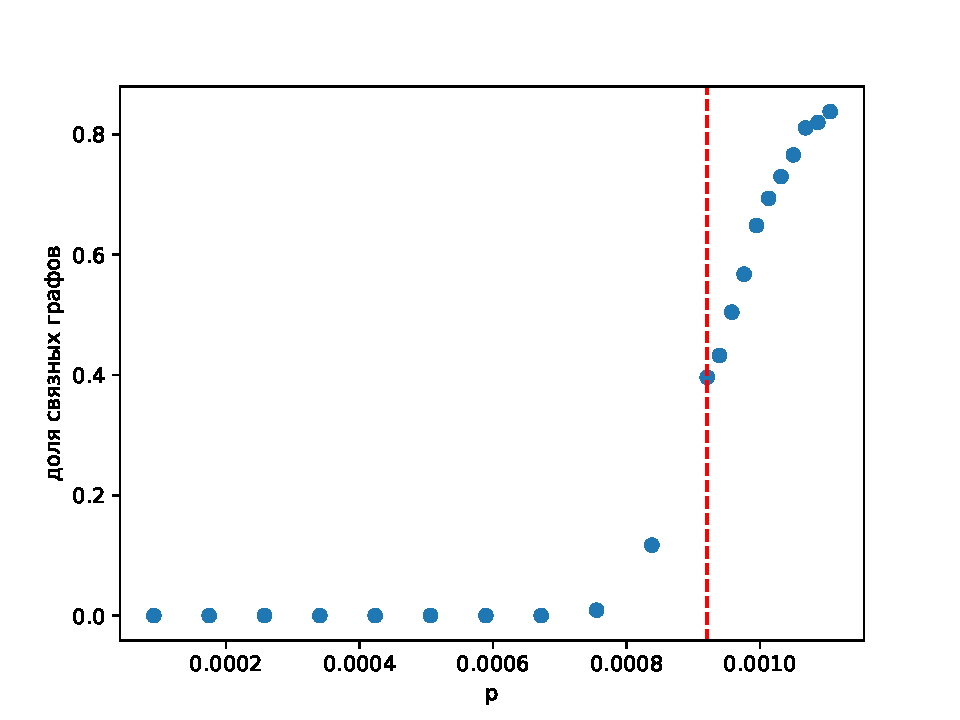
\includegraphics{../../plots/connected.pdf} 
    \caption{Изменение доли связных графов при $p \in [0.1 \frac{\ln{n}}{n};1.2 \frac{\ln{n}}{n}]$}
    \label{con}
\end{figure}  
На рисунке \ref{con} можно заметить фазовый переход 
$p = \frac{\ln{n}}{n}$. Структура построенных графов меняется 
при достижении этого значения.
\subsection{Исследование структуры графов}
Структура графа была исследована путем расчета доли 
деревьев среди всех компонент связности графа. Были проведены 
153 эксперимента, вычислена средняя доля деревьев среди всех экспериментов, $n=10000$, $\epsilon=0.1$.
\begin{figure}[H] 
\centering 
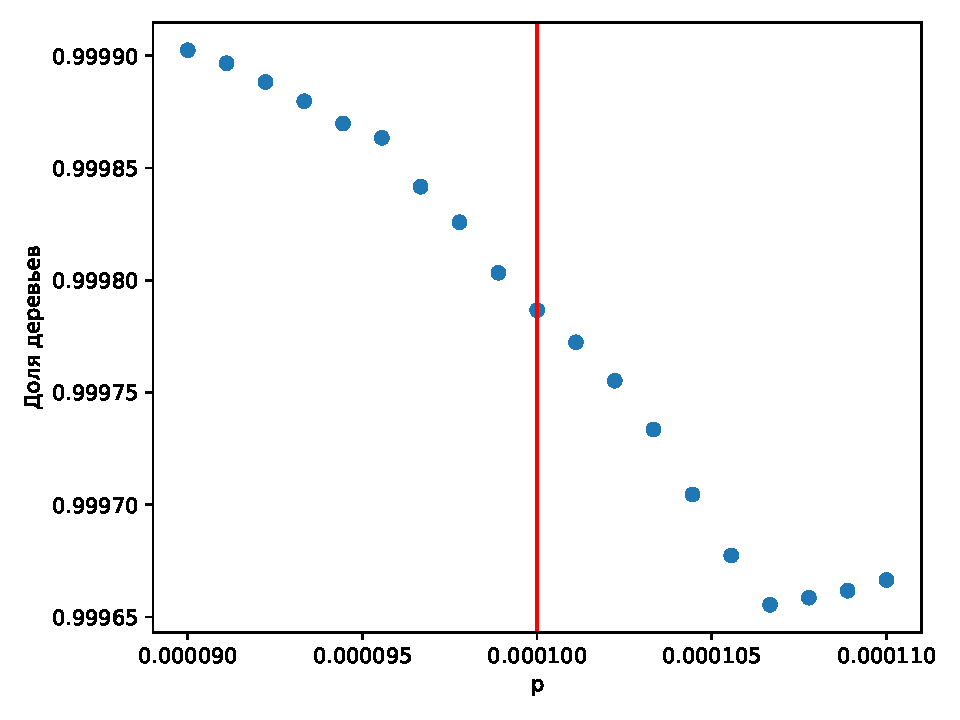
\includegraphics[scale=0.8]{../../plots/tree1.pdf}
\caption{Изменение доли деревьев при $p \in [\frac{1-\epsilon}{n};\frac{1+\epsilon}{n}]$}
\label{tree_1}
\end{figure} 
\begin{figure}[H] 
\centering 
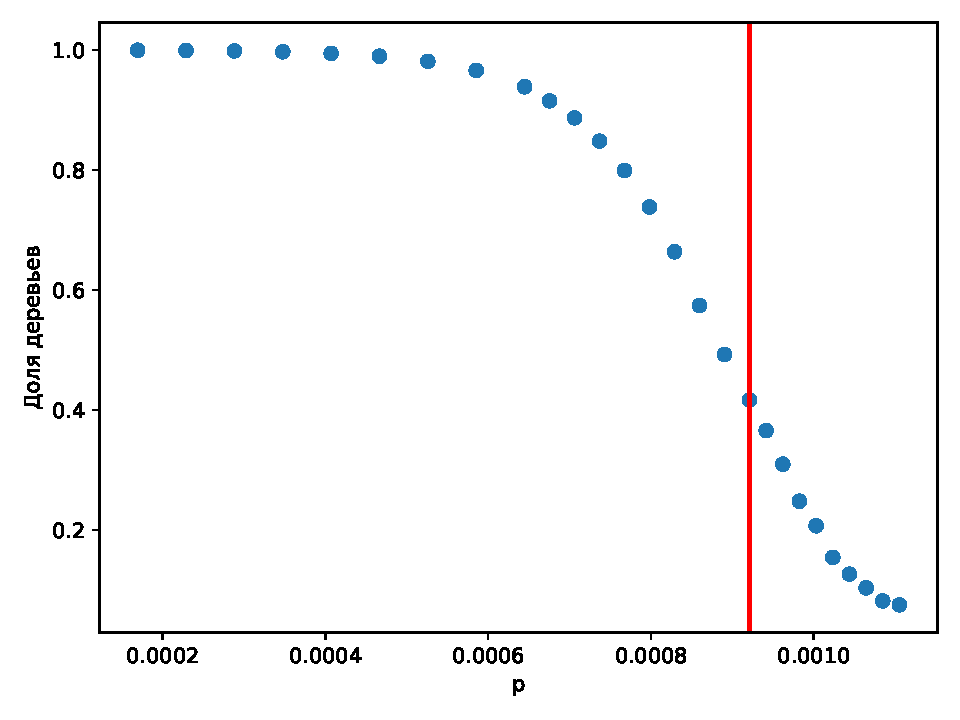
\includegraphics[scale=0.8]{../../plots/tree2.pdf}
\caption{Изменение доли деревьев при $p \in [\frac{1+\epsilon}{n};1.1 \frac{\ln{n}}{n}]$}
\label{tree_2}
\end{figure} 

Из рисунков \ref{tree_1},\ref{tree_2} 
можно заметить, как меняется структура графа. До 
первого фазового перехода $p = \frac{1}{n}$, в графе 
были в основном деревья, после него появилась гигантская компонента связности, которая деревом не является. После второго фазового перехода $p =\frac{\ln{n}}{n}$ в виде деревьев остались немногочисленные изолированные вершины.
